\documentclass{../template/texnote}

\title{\textbf{Introduction to Solar Astronomy}}[author={Linn Abraham}]

\begin{document}
    \maketitle \currentdoc{note}
    %<*note>

\section{The Sun is Exciting to Study}
Being the star that is closest to us, the Sun is the best laboratory to expand our understanding about stars and stellar processes in general.
It is what drives our ambitious goal of unlocking the ultimate source of power, i.e, controlled fusion reaction.
Which is capable of provding clean energy for the entire known future of humanity.
It can help us learn about neutrinos and several more fascinating things.
It is also the heavenly body that has the greatest influence on earth. From the harmless aurorae to geomagnetic storms that are capable of deorbiting satellites and 
temporary power grid failures.
There are a a lot of questions that remains answered about the Sun.
What heats up the corona to such high temperatures, What triggers flaring activities in the Sun etc.
India now has it's own space based solar observatory with Aditya-L1. Several of the instruments open a never before seen window on the Sun.

%\section{Milestones in our Understanding about the Sun}
\subsection{Sunspots}
The surface of the Sun reveals that it is not a perfect orb as expected of a heavenly body acoording to a divine picture of creation.
This fact was discovered by Galileo amongst others as soon as he trained the latest invention of the day, the telescopes,  towards these heavenly bodies \ref{fig:sunspot}.
         %Sunspots were historically one of the most prominent features observed about our Sun. 
         %Soon after the discovery of the telescope, Galileo and others pointed it towards the Sun and observed these blemishes on the Sun's surface.
         Note that these observations are not made directly but by projecting it onto a screen and often making drawings of what was sceen.
With the limited knowledge about the Sun they had at the time, many considered them to be other planets or as slag of the burning Sun or even opaque smoke clouds.
It was soon discovered that there is a cyclic pattern to the appearance and disappearance of Sunspots.
An observation that has finally lead to the coinage ``solar cycle'' denoting the periodic magnetic activity in the Sun.
The Sun being crucial to life on Earth, this cycle can also be seen as fundamental cycle of nature. 
The popular science book ``Nature's Third Cycle'' by Dr. Arnab Rai Choudhury explores this concept in great detail.

\begin{figure}[htpb]
    \centering
    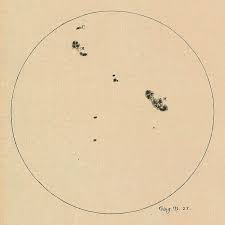
\includegraphics[width=0.48\textwidth]{Linn/sunspot_galileo_single.jpeg}
    \caption{Original drawing of Sunspots made by Galileo.} 
    \label{fig:sunspot}
\end{figure}

\subsection{Corona}
The solar corona was photographed for the first time during a solar eclipse. It is the halo of light with long strands and intricate pattern seen during a total solar eclipse of the Sun when the moon blocks the light coming from the Sun's disk. 
The corona expands into the interplanetary space and beyond in the form of the solar wind.
You may be familar with the grand display of colours that happens in the skies above the northern and southern poles known as Aurorae.
This happens as a result of the interaction of the solar wind with the Earth's own magnetic field.
\begin{figure}[htpb]
    \centering
    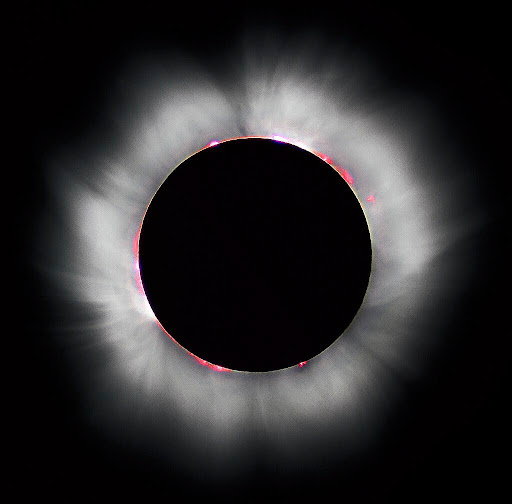
\includegraphics[width=0.48\textwidth]{Linn/corona.jpg}
    \caption{Corona as observed during a total solar eclipse.} 
    \label{fig:corona}
\end{figure}

\section{What can we learn about the Sun?} 
\subsection{Interior of the Sun vs. The Solar Atmoshpere}
It can be seen from theoretical calculations that the matter in the interior of the Sun should exist in the plasma state of matter. 
However by calculating the mean free path inside the Sun and the sizes of the constituent particles it can be seen that the plasma in the Sun
behaves like a perfect gas.
%The interior of the Sun is not directly observable.
Considering the densities and temperatures inside the Sun it can be seen that most of the Sun's interior is opaque. 

%\subsection{Atmoshpere of the Sun}
The part of the Sun from which photons can directly escape into space is called the atmosphere of the Sun.
It consists of the Photosphere, Chromosphere and Corona.
The part of the Sun that is directly visible to us is called the Photosphere.
It is interesting to note that the high energy gamma rays generated by nuclear fusion in the Sun's core takes 1,70,000 years to reach the photosphere. Where the collisions brings the wavelength into the visible regime.

%\section{How do we know about the Sun?}
\section{Shedding Light on the Sun}
We obviously know about the Sun by observations in the visible spectrum. 
Or in other words observations made in the visible region of the spectrum are looking into the photosphere of the Sun.
Being the blackbody that the Sun is, we also expect it to emit in other wavelengths.


\subsection{How magnetic fields complicates things}
The presence of high magnetic fields on the Sun's surface were first observed by spectroscopic analysis.
Specifically the Zeeman splitting of spectral lines allows us to gauge the presence and strength of magnetic field through which light has passed before reaching the detector.
Using the Zeeman effect it was also found that Sunspots are regions of higher magnetic field than surrounding regions.
The presence of magnetic field is unavoidable once we understand that plasma which the Sun is made up of is essentially a soup of charged ions and electrons.
And we know that moving charges always create magnetic field.
However since plasma is also neutral if you consider both charges together, it is not that simple to explain.
Our best understanding of the mechanism behind the magnetic field generation is called the Dyanamo model.

The presence of magnetic fields means that the Sun's emission can no longer be understood just as a black body emission.
One observation that shows how magentic fields can complicate things is the nature of temperature distribution in the Solar atmosphere.
The temperature in the solar atmosphere instead of decreasing with height, stop decreasing when it reaches the region known as the transition regions and then rapdily shoots up. Reaching 1 million in the corona. This is called the coronal heating problem.
The presence of such high temperature leads to the presence of several emission lines in the UV and X-ray regions.

\section{Features and Events on the Sun}
\subsection{Active Regions}
The other way in which magnetic field complicates things is by producing active regions that are probable to produce prominences, flares, CMEs etc.
An active region by definition is a region of complex magnetic field and is produced as a result of the twisting of magnetic field due to the solar differential rotation as well the convection currents and other dynamics in the Sun's interior.
When an active region matures we find within it darker regions of more intense magnetic field that are the Sunspots.
Near to these active regions one can often find cool dark ribbons called filaments (when observed on disc) and prominences (when observed against the limb).
Such prominence are prone to eruption at some point in their lifetime resulting at times in a CME or sometimes in a solar flare.
CMEs involve mass being ejected into the space surrounding the Sun whereas flares are intense violet release of energy as radiation.
\begin{figure}[htpb]
    \centering
    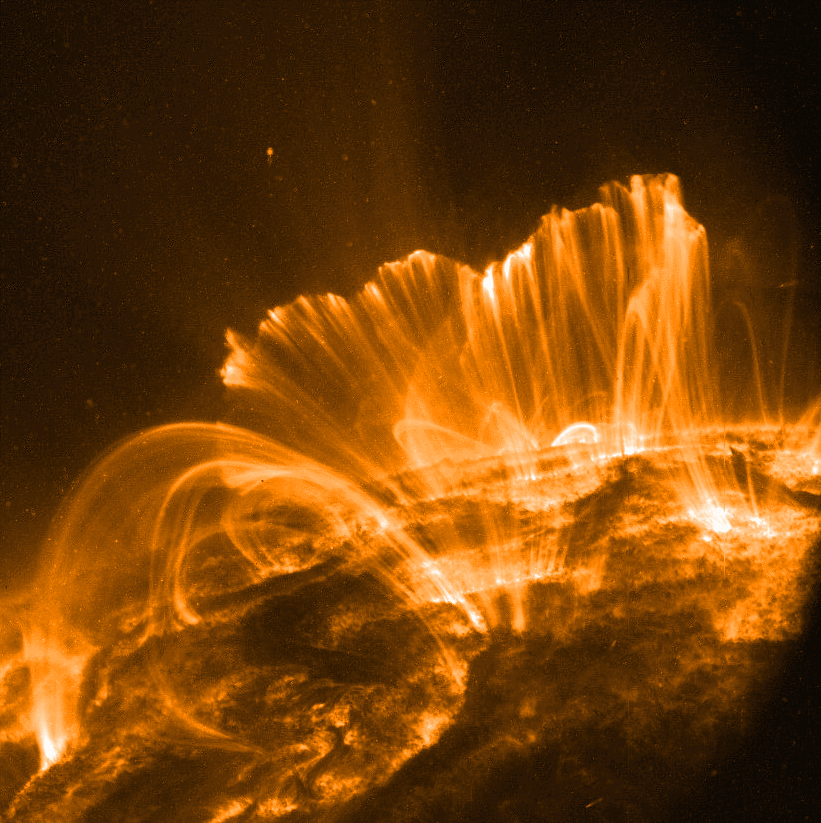
\includegraphics[width=0.48\textwidth]{Linn/solar_flare_trace.png}
    \caption{Post-eruptive loops in the wake of a solar flare, image taken by the TRACE satellite (photo by NASA)} 
    \label{fig:flare}
\end{figure}

\section{How best to study the Sun?}
There are several methods to study the Sun depending on your specific interest.
For example if you are interested in learning about flares, there are some flares that are observable in the visible region of the EM spectrum, that are called white light flares.
There are ground and space based instruments that may be able to detect the X-ray particles emitted as part of these flares. 
Usually the detections are done separately in the soft and hard X-ray channels.
Such instruments are often used to detect whether a flare has happened or not and since they mostly integrate the x-ray emission over the whole disc of the Sun, the location information would be lost for where the flare has occurred.
We mentioned the possibility of using the Zeeman effect to quantify the magnetic field in the Sun. % wher in the Sun?
In fact it is possible to build a map of the Sun using this magnetic field measurement.
Such a map in which the areas of strong positive magnetic field are colored white, the strong negative magnetic field regions are colored black and grey regions show areas with an absence of magnetic fields.
Coronographs are used to continously observe the Corona by artificially eclisping the Sun with the help of an occulting disc. 
The light obtained using this can be further subjected to spectroscopic analysis.
\begin{figure}[htpb]
    \centering
    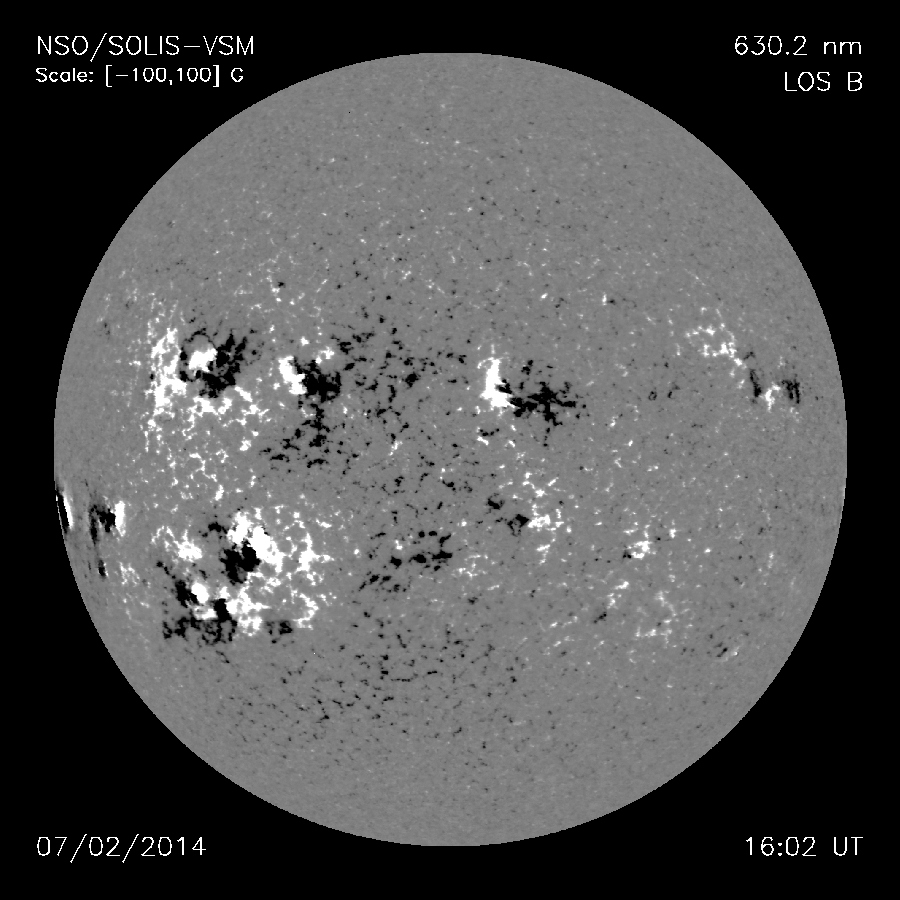
\includegraphics[width=0.48\textwidth]{Linn/magnetogram.jpg}
    \caption{NISP/SOLIS magnetogram from 18 June 2014 during solar maximum.} 
    \label{fig:magnetogram}
\end{figure}


\subsection{Imaging in the Ultraviolet}

We had already mentioned that at different heights in the solar atmosphere you have different temperatures.
By imaging the Sun in narrow passbands centered over wavelengths in the Ultraviolet region, we are effectively looking into the Solar atmosphere at 
different heights.
This is because the temperatures present at the different layers leads to specific ionizations that emit in specific wavelengths in the Ultraviolet region.
Spectroscopy is often time consuming and leads to low cadence data.
However we can obtain a very high cadence when using imaging and this is specially relevant for changes in the solar surface that happen at very small time scales.
Ultraviolet being abosrbed to a high extent by the Earth's atmosphere we need space based telescope for such observations.
Existing space based solar observatories like the Solar Dynamic Observatory (SDO) have given us valuable data over the year and is still observing the Sun.
India has it's own space based solar observatory called Aditya-L1 which carries the Solar Ultraviolet Imaging Telescope (SUIT) developed by the Inter University Center for Astronomy and Astrophysics (IUCAA) along with many other institutions across India.
In comparison to the Atmospheric Imaging Assembly (AIA) telescope onboard SDO which images the Sun primarily in 7 Extreme Ultraviolet (EUV) channels, SUIT observes the Sun in 8 Near Ultraviolet (NUV) channels. 
\begin{figure}
    \centering
    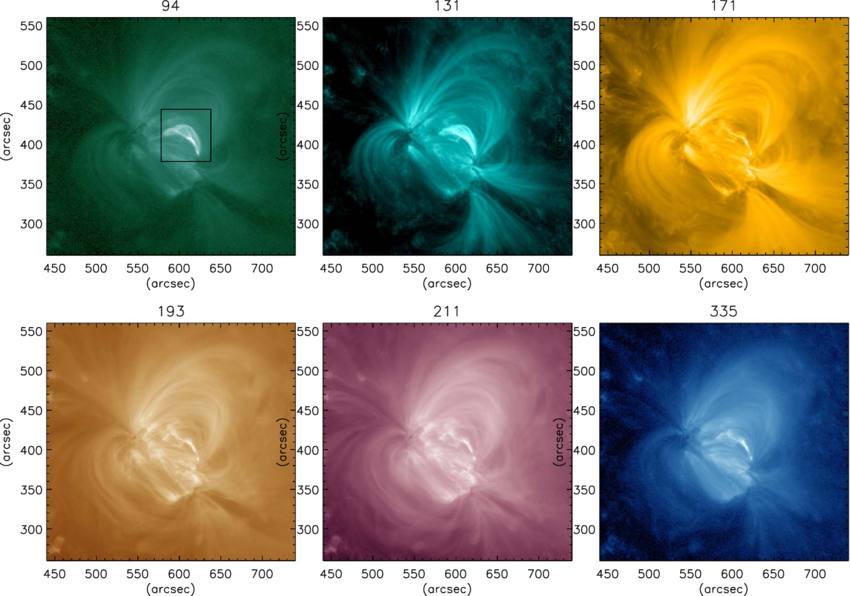
\includegraphics[width=0.48\textwidth]{Linn/AIA.png}
    \caption{The SDO/AIA images observed in multiwavelength channels targeting the AR 12804 observed on 2021 February 25 at flare peak time (14:16 UT).} 
    \label{fig:AIA}
\end{figure}

%\nocite{choudhuri_natures_2015}
%\nocite{shu_physical_1982}
%\nocite{priest_magnetohydrodynamics_nodate}
%\nocite{lemen_atmospheric_2012}

%\begin{thebibliography}{4}
%\providecommand{\natexlab}[1]{#1}
%\providecommand{\url}[1]{\texttt{#1}}
%\expandafter\ifx\csname urlstyle\endcsname\relax
%  \providecommand{\doi}[1]{doi: #1}\else
%  \providecommand{\doi}{doi: \begingroup \urlstyle{rm}\Url}\fi
%\bibitem[1]{choudhuri_natures_2015}
%Arnab~Rai Choudhuri.
%\newblock \emph{Nature's Third Cycle: A Story of Sunspots}.
%\newblock {Oxford University Press}, {Oxford ; New York}, 2015.
%\newblock ISBN 978-0-19-967475-6.
%
%\bibitem[2]{shu_physical_1982}
%Frank~H. Shu.
%\newblock \emph{The Physical Universe: An Introduction to Astronomy}.
%\newblock A Series of Books in Astronomy. {Univ. Sience Books}, {Sausalito,
%  Calif}, 9. print edition, 1982.
%\newblock ISBN 978-0-935702-05-7.
%
%\bibitem[3]{priest_magnetohydrodynamics_nodate}
%Eric Priest.
%\newblock Magnetohydrodynamics of {{The Sun}}.
%
%%\bibitem[4]{lemen_atmospheric_2012}
%%James~R. Lemen, Alan~M. Title, David~J. Akin, Paul~F. Boerner, Catherine Chou,
%%  Jerry~F. Drake, Dexter~W. Duncan, Christopher~G. Edwards, Frank~M.
%%  Friedlaender, Gary~F. Heyman, Neal~E. Hurlburt, Noah~L. Katz, Gary~D.
%%  Kushner, Michael Levay, Russell~W. Lindgren, Dnyanesh~P. Mathur, Edward~L.
%%  McFeaters, Sarah Mitchell, Roger~A. Rehse, Carolus~J. Schrijver, Larry~A.
%%  Springer, Robert~A. Stern, Theodore~D. Tarbell, Jean-Pierre Wuelser, C.~Jacob
%%  Wolfson, Carl Yanari, Jay~A. Bookbinder, Peter~N. Cheimets, David Caldwell,
%%  Edward~E. Deluca, Richard Gates, Leon Golub, Sang Park, William~A. Podgorski,
%%  Rock~I. Bush, Philip~H. Scherrer, Mark~A. Gummin, Peter Smith, Gary Auker,
%%  Paul Jerram, Peter Pool, Regina Soufli, David~L. Windt, Sarah Beardsley,
%%  Matthew Clapp, James Lang, and Nicholas Waltham.
%%\newblock The {{Atmospheric Imaging Assembly}} ({{AIA}}) on the {{Solar
%%  Dynamics Observatory}} ({{SDO}}).
%%\newblock \emph{Solar Physics}, 275\penalty0 (1-2):\penalty0 17--40, January
%%  2012.
%%\newblock ISSN 0038-0938, 1573-093X.
%%\newblock \doi{10.1007/s11207-011-9776-8}.
%
%\end{thebibliography}
\vspace{0.5cm}
\noindent\fbox{%
	\parbox{\textwidth}{%
		\textbf{About the Author}\vspace{0.2cm} \\
		\textbf{Linn Abraham} is a researcher in Physics, specializing in A.I. applications to astronomy. 
He is currently involved in the development of CNN based Computer Vision tools for
prediction of solar flares from images of the Sun, morphological classifications of galaxies from optical images surveys and radio galaxy source extraction from radio observations.
	}
}
    %</note>
    \printbibliography
\end{document}
